% !TeX root = ../master.tex

\lecture{8}{2026-09-17}{Svigtkriterier}

\section{Svigtkriterier}
Vi har tidligere brugt bl.a. Von Mises som svigtkriterie, dette er \textit{ikke} brugbart for kompositter.
Dette skyldes bl.a. at Von Mises forudsætter at materialet er isotropt og duktilt, hvilket ikke gælder for kompositter.
Sprøde materialer som kompositter forudsætter derimod brugen af en af flere andre svigtkriterier, hvoraf nogle i det følgende vil blive gennemgået.
I dette kursus vil vi arbejde med:
\begin{itemize}
  \item Maksimal spænding
  \item Maksimal tøjning
  \item Tsai-Wu
  \item Tsai-Hill
\end{itemize}
Der findes også et væld af andre såsom \textit{Hill}, \textit{Hoffman}, \textit{Puck}, \textit{Cuntze}, \textit{Hashin}, \textit{Hart-Smith}, omend disse ikke vil blive gennemgået.
Ingen af svigtkriterierne er perfekte og de har alle forskellige fordele og ulemper.

I svigtkriterier bruges $X$ for styrker i fiberretningen, $Y$ for styrker på tværs af fiberretningen og $S$ for shear.

\subsection{Maksimal spænding}
For maksimal spænding antager vi at svigt sker når en af følgende uligheder bliver brudt:
\begin{equation*}
  \sigma_1 < X_t \quad \sigma_2 < Y_t, \quad \sigma_1 > X_c, \sigma_2 > Y_x, \left| \tau_{12} \right| < S
.\end{equation*}
\textit{Failure Envelopen} for svigtkriteriet for maksimal spænding er vist på \Mref{fig:maxstressenvelope}.

\begin{figure} [ht]
  \centering
  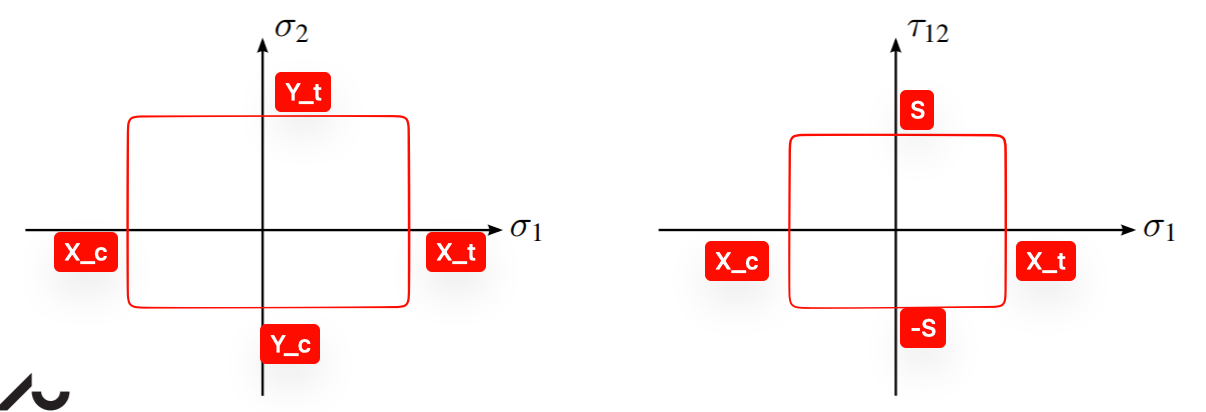
\includegraphics[width=0.8\linewidth]{./figures/maxstressenvelope.png}
  \caption{\textit{Failure Envelope} for maksimalspændings svigtkriteriet.}
  \label{fig:maxstressenvelope}
\end{figure}

Som også fremgår af \Mref{fig:maxstressenvelope} så fås der nogle ``hjørner'' på failure envelopen der er ufysiske -- man kan ikke praktisk regne med at sætte $\sigma_1 = X_t$ og $\sigma_2 = Y_t$ uden svigt idet det to retninger vil forstærke hinanden i nogen grad, omend dette ikke er beskrevet af svigtkriteriet.


\subsection{Maksimal Tøjning}
Når vi arbejder med maksimal tøjning benytter vi i stedet en foreskrevet maksimal tøjning $X_{\epsilon}, Y_{\epsilon}, S_{\epsilon}$.
For maksimal tøjning svigtkriteriet antager vi at svigt sker når en af følgende uligheder ikke overholdes:
\begin{equation*}
  \epsilon_1 < X_{\epsilon t}, \quad \epsilon_2 < Y_{\epsilon t}, \quad \epsilon_{1} > X_{\epsilon c}, \quad \epsilon_2 > Y_{\epsilon c}, \quad \left| \gamma_{12} \right| < S_{\epsilon} 
.\end{equation*}
Her vil vi få en failure envelope der ligner den fra \Mref{fig:maxstressenvelope} og den vil have de samme svagheder med specielt bi-aksielle tøjningssituationer.
I det en lineær spændings-tøjningsrelation antages fås:
\begin{equation*}
  X_{\epsilon t} = \frac{X_t}{E_1}, \quad Y_{\epsilon t} = \frac{Y_t}{E_2}, \quad X_{\epsilon c} = \frac{X_c}{E_1}, \quad Y_{\epsilon c} = \frac{Y_c}{E_2}, \quad S_{\epsilon} = \frac{S}{G_{12}}
.\end{equation*}

\subsection{Tsai-Hill}
Her antager vi planspænding og lineær-elastisk opførsel.
Tsai-Hill minder mere om Von Mises end de ovenstående idet vi også her kun får et kriterie.
Her har vi at svigt sker når:
\begin{equation*}
  \frac{\sigma_1^2}{X^2} - \frac{\sigma_1 \sigma_2}{X^2} + \frac{\sigma_2^2}{Y^2} + \frac{\tau_{12}^2}{S^2} < 1
.\end{equation*}
Denne søger mod at tage højde for nogle af svaghederne ved maksimal spænding og tøjning specielt ift. biaksiel belastning.
Tsai-Hill skelner ikke mellem tryk- og træk-styrker, hvilket er en stor svaghed.
Den undervurderer også svigtspæænding fordi $Y_t$ er mindre for et UD-lamina end $Y_c$.

Failure envelopen for Tsai-Hill er vist på \Mref{fig:tsai-hill}.

\begin{figure} [ht]
  \centering
  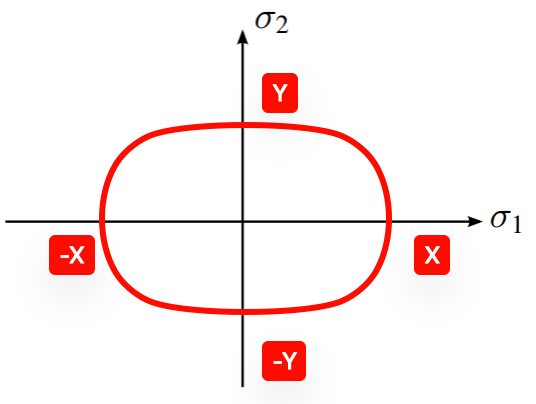
\includegraphics[width=0.6\linewidth]{./figures/tsai-hill.png}
  \caption{Failure-Envelope for Tsai-Hill}
  \label{fig:tsai-hill}
\end{figure}

\subsection{Tsai-Wu}
Her antages ligeledes planspænding for et ortotropisk lamina.
Følgende ulighed er gældende for Tsai-Wu:
\begin{equation*}
  F_1 \sigma_1 + F_2 \sigma_2 + F_6 \tau_{12} + F_{11} \sigma_1^2 + F_{22} \sigma_2^2 + F_{66}\tau_{12}^2 + 2 F_{12} \sigma_1 \sigma_2 < 1
\end{equation*}
hvor $F_1, F_2, F_6, F_{11}$ og $F_{22}$ er defineret som:
\begin{equation*}
  F_1 = \frac{1}{X_t} + \frac{1}{X_c}, \quad F_2 = \frac{1}{Y_t} + \frac{1}{Y_c},  \quad F_{11} = -\frac{1}{X_t X_c}, \quad F_{22} = - \frac{1}{Y_t Y_c}, \quad F_6 = 0, \quad F_{66} = \frac{1}{S^2}
.\end{equation*}
Den nye parameter $F_{12}$ er en uafhængig interaktionsparameter, der er svær at bestemme hvorfor en biaksiel test er nødvendig.
Stephen Tsai forelsår at sætte $F_{12}^{*} = \num{-0,5}$ i
\begin{equation*}
  F_{12} = F_{12}^{*} \sqrt{F_{11} F_{22}}
.\end{equation*}

Denne har bedre fitting end de øvrige grundet $F_{12}$ og inkluderer interaktionen mellem forskellige modes. Derudover er den repræsenteret ved kun en enkelt ligning som Tsai-Hill.
Ulemperne ved Tsai-Wu kan være at det er mere ala curve-fitting end egentlig brugbar svigtdata, da $F_{12}$ kan være enormt svær at bestemme.
Tsai-Hill, Tsai-Wu og deres afledte overvurderer generelt den biaksielle kompressionsstyrke med op til en faktor 3.
For at undgå dette kan man vælge at kombinere forskellige svigtkriterier således at et andet kriterie end Tsai-Hill/Tsai-Wu benyttes for biaksiel kompression.
Failure envelopen her vil blive en ``aflanget oval''.
